\documentclass[sans]{beamer}

\usepackage{lmodern}
\usepackage{tikz}
\usepackage{pdfpages}
%\usepackage{overpic}
\usetikzlibrary{arrows, positioning, shapes.geometric}
\usetikzlibrary{shadows.blur}

% hide the footline navigation
\setbeamertemplate{footline}[frame number]{}
\setbeamertemplate{navigation symbols}{}
\setbeamertemplate{footline}{}

\tikzset{
    %Define standard arrow tip
    >=stealth',
}


%
%     % Define arrow style
%     pil/.style={
%         ->,
%         thick,
%         shorten <=2pt,
%         shorten >=2pt,
%     }
% }

\tikzset{
    invisible/.style={opacity=0,text opacity=0},
    visible on/.style={alt=#1{}{invisible}},
    alt/.code args={<#1>#2#3}{%
      \alt<#1>{\pgfkeysalso{#2}}{\pgfkeysalso{#3}}
    },
}

\tikzset{
  setstyle/.style={#1},
  %bcg/.default={white},
  setstyle on/.style={alt=#1{}{setstyle}},
}

\tikzset{
  background fill/.style={fill=#1},
  background fill/.default={white},
  fill on/.style={alt=#1{}{background fill}},
}

\tikzset{
  background draw/.style={draw=#1},
  background draw/.default={white},
  draw on/.style={alt=#1{}{background draw}},
}

\tikzset{
  background filldraw/.style 2 args={draw=#1, fill=#2},
  background filldraw/.default={white}{white},
  filldraw on/.style={alt=#1{}{background filldraw}},
}

\tikzset{
  background shade/.style={#1},
  background shade/.default={top color=white, bottom color=white},
  shade on/.style={alt=#1{}{background shade}},
}

\tikzset{
  background shadedraw/.style 2 args={draw=#1, #2},
  background shadedraw/.default={white}{top color=white, bottom color=white},
  shadedraw on/.style={alt=#1{}{background shadedraw}},
}

\begin{document}
  \centering
  %\frametitle{This is the first slide}
  \begin{frame}
  %\fontsize{1cm}{0.5cm}{\textbf{SYMBIOTIC \textcolor{red}{3}}}
  \huge{\textbf{SYMBIOTIC \textcolor{red}{3}}}\\
  \vspace{0.3cm}
  \large{NEW SLICER AND ERROR-WITNESS GENERATION}
   \vspace{1cm}

    \underline{Marek~Chalupa}, Martin~Jon\'{a}\v{s}, Jiri~Slaby,\\
    Jan~Strej\v{c}ek, and Martina Vitovsk\'{a}

     \vspace{1cm}
   Masaryk University, Brno
  \end{frame}

  \begin{frame}
  \frametitle{Symbiotic workflow}

    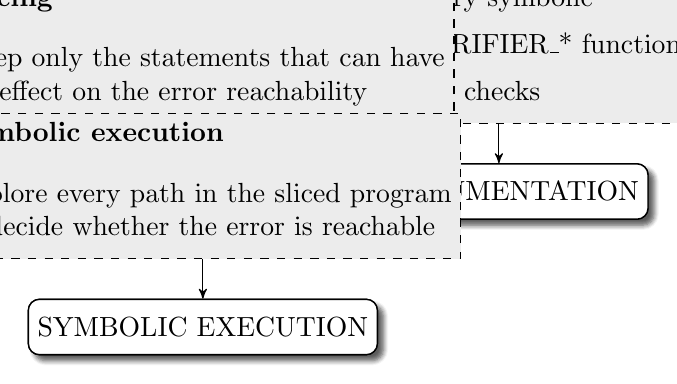
\begin{tikzpicture}
    	\tikzset{
	  wn/.style={draw, fill=white,
	             %line width=1pt,
		     minimum height=2em,
	             %shade,
	             shape=rectangle,
		     line width=0.5pt,
		     rounded corners},
	 shd/.style={blur shadow={shadow blur steps=5}}
	},

    	\node [wn, shd, ] (sources) {SOURCES};
    	\node [wn, shd, right =of sources] (llvm) {LLVM};
    	\alt<2>{\node[wn, shd, below =of llvm, fill=yellow] (instr) {INSTRUMENTATION};}
	         {\node[wn, shd, below =of llvm] (instr) {INSTRUMENTATION};}
    	\alt<3>{\node [wn, shd, left =of instr, fill=yellow] (slicing) {SLICING};}
    	       {\node [wn, shd, left =of instr] (slicing) {SLICING};}
    	\alt<4>{\node [wn, shd, below =of slicing, fill=yellow] (se) {SYMBOLIC EXECUTION};}
    	       {\node [wn, shd, below =of slicing] (se) {SYMBOLIC EXECUTION};}

        \path[draw,->] (sources) edge (llvm)
	               (llvm) edge (instr)
		       (instr) edge (slicing)
		       (slicing) edge (se);

        %% text boxes over the imge
        \tikzset{overlaybox/.style={draw=black, minimum width=2em,
	                            fill=gray!15, align=left,
                                    dashed, overlay, text depth=5,
                                    opacity=1}}
    	\node<2>[above =0.5cm of instr, overlaybox] (float1)
                  {\textbf{Instrumentation}\\[1em]
                    Make memory symbolic\\[0.5em]
                    Define \_\_VERIFIER\_* functions\\[0.5em]
                    Insert errors checks
                   };

    	\node<3>[above =0.5cm of slicing, overlaybox] (float2)
                  {\textbf{Slicing}\\[1em]
                    Keep only the statements that can have\\
                   an effect on the error reachability
                   };

    	\node<4>[above =0.5cm of se, overlaybox] (float2)
                  {\textbf{Symbolic execution}\\[1em]
                   Explore every path in the sliced program\\
                   to decide whether the error is reachable
                   };

       %\definecolor{dgreen}{rgb}{125,255,125}
      %\only<5>{
      %  % create fade on everything except INSTR and SLICING
      %  \node[above = 0.2cm of instr, fill=white, opacity=0.7,
      %        overlay, text width= 10cm, text depth = 2cm] (white1) {};

      %  \node[below = 0.2cm of slicing, fill=white, opacity=0.7,
      %        overlay, text width= 10cm, text depth = 2cm] (white1) {};

      % % colorize the INST and SLICING
      % \node[wn, shd, below =of llvm, fill=red!50] (instr) {INSTRUMENTATION};
      % \node [wn, shd, left =of instr, fill=red!50] (slicing) {SLICING};
      %}

      %\only<5-6> {
      %  \node[above = 0.2cm of slicing] (llvmslicer) {llvm-slicer};
      %  \node[above = 0.2cm of instr] (opt) {opt};
      %  \node[above = 0.2cm of se] (klee) {KLEE + \textcolor{red}{witnesses}};
      %}

      %\only<6>{
      %  \node[above = 0.2cm of slicing] (llvmslicer) {llvm-slicer};
      %  \node[above = 0.2cm of instr] (opt) {opt};
      %  \node[above = 0.2cm of se] (klee) {KLEE + witnesses};

      % \node [wn, shd, right =of sources, fill=orange!50] (llvm) {LLVM};
      % \node[wn, shd, below =of llvm, fill=yellow!50] (instr) {INSTRUMENTATION};
      % \node [wn, shd, left =of instr, fill=green!50] (slicing) {SLICING};
      % \node [wn, shd, below =of slicing, fill=blue!50] (se) {SYMBOLIC EXECUTION};

      % %\node [below =of instr, rotate=27] (modul) {\huge{MODULARITY!}};
      %}

    \end{tikzpicture}

  %More content goes here
  \end{frame}

  \begin{frame}
  \frametitle{Symbiotic - what we did}

    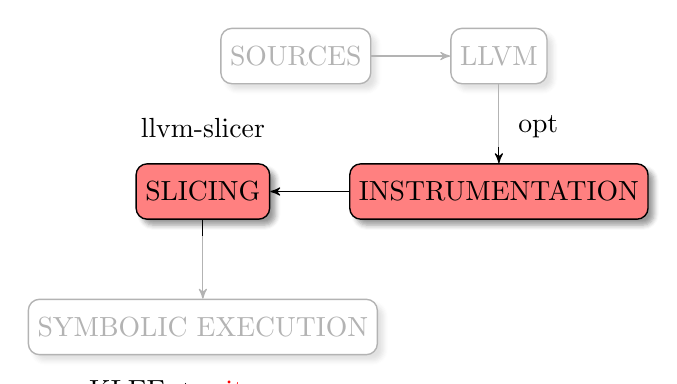
\begin{tikzpicture}
    	\tikzset{
	  wn/.style={draw, fill=white,
	             %line width=1pt,
		     minimum height=2em,
	             %shade,
	             shape=rectangle,
		     line width=0.5pt,
		     rounded corners},
	 shd/.style={blur shadow={shadow blur steps=5}}
	},

    	\node [wn, shd, ] (sources) {SOURCES};
    	\node [wn, shd, right =of sources] (llvm) {LLVM};
	\node[wn, shd, below =of llvm, fill=red!50] (instr) {INSTRUMENTATION};
    	\node [wn, shd, left =of instr, fill=red!50] (slicing) {SLICING};
        \node [wn, shd, below =of slicing] (se) {SYMBOLIC EXECUTION};

        \path[draw,->] (sources) edge (llvm)
	               (llvm) edge (instr)
		       (instr) edge (slicing)
		       (slicing) edge (se);

         % create fade on everything except INSTR and SLICING
         \node[above = 0.2cm of instr, fill=white, opacity=0.7,
	       overlay, text width= 10cm, text depth = 2cm] (white1) {};

         \node[below = 0.2cm of slicing, fill=white, opacity=0.7,
	       overlay, text width= 10cm, text depth = 2cm] (white1) {};

	 \node[above = 0.2cm of slicing] (llvmslicer) {llvm-slicer};
	 \node[above = 0.2cm of instr, xshift=0.5cm] (opt) {opt};
	 \node[below = 0.2cm of se, overlay] (klee) {KLEE + \textcolor{red}{witnesses}};

    \end{tikzpicture}

  %More content goes here
  \end{frame}

  \begin{frame}
  \frametitle{Symbiotic - modularity}

    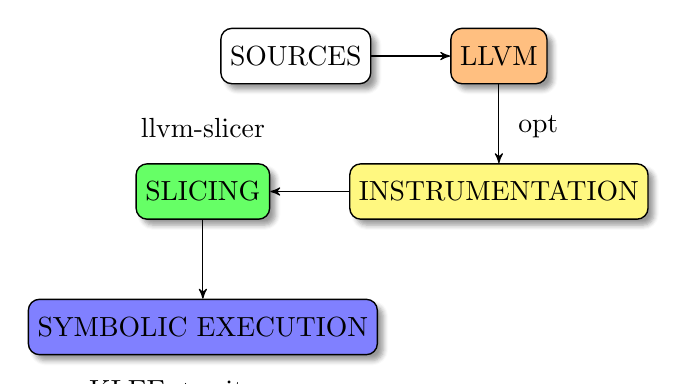
\begin{tikzpicture}
    	\tikzset{
	  wn/.style={draw, fill=white,
	             %line width=1pt,
		     minimum height=2em,
	             %shade,
	             shape=rectangle,
		     line width=0.5pt,
		     rounded corners},
	 shd/.style={blur shadow={shadow blur steps=5}}
	},

    	\node [wn, shd, ] (sources) {SOURCES};
    	\node [wn, shd, right =of sources, fill=orange!50] (llvm) {LLVM};
	\node[wn, shd, below =of llvm, fill=yellow!50] (instr) {INSTRUMENTATION};
    	\node [wn, shd, left =of instr, fill=green!60] (slicing) {SLICING};
        \node [wn, shd, below =of slicing, fill=blue!50] (se) {SYMBOLIC EXECUTION};

        \path[draw,->] (sources) edge (llvm)
	               (llvm) edge (instr)
		       (instr) edge (slicing)
		       (slicing) edge (se);

	 \node[above = 0.2cm of slicing] (llvmslicer) {llvm-slicer};
	 \node[above = 0.2cm of instr, xshift=0.5cm] (opt) {opt};
	 \node[below = 0.2cm of se, overlay] (klee) {KLEE + witnesses};

    \end{tikzpicture}

  %More content goes here
  \end{frame}

  \begin{frame}
  \frametitle{Measurements}
  \framesubtitle{Effect of slicing}
  \begin{figure}
  \includegraphics[height=7.2cm]{slicing_effect1.pdf}
  \end{figure}

  \end{frame}

  \begin{frame}
  \frametitle{Measurements}
  \framesubtitle{Slicing speed}
  %\includegraphics[height=8cm]{histtime.pdf}
  \includegraphics[height=8cm]{histtime.pdf}
  \end{frame}

  \begin{frame}
  \frametitle{Measurements}
  \framesubtitle{Size of sliced flow-graph}
  \begin{figure}
  \includegraphics[height=8cm]{histnodes.pdf}
  \end{figure}
  \end{frame}

% \begin{frame}
% \frametitle{Measurements}
% \framesubtitle{(Size of sliced module - DELETE?)}
% \begin{figure}
% \includegraphics[height=8cm]{histmod.pdf}
% \end{figure}
% \end{frame}

  \begin{frame}
  \textcolor{blue}{\url{https://github.com/staticafi/symbiotic}}\\[1em]
  \huge{Thank you for your attention!}
  \end{frame}

% etc
\end{document}
